\documentclass[pdflatex,sn-mathphys-num]{sn-jnl}

\usepackage{graphicx}
\usepackage{multirow}
\usepackage{amsmath,amssymb,amsfonts}
\usepackage{amsthm}
\usepackage{mathrsfs}
\usepackage[title]{appendix}
\usepackage{xcolor}
\usepackage{textcomp}
\usepackage{manyfoot}
\usepackage{booktabs}
\usepackage{algorithm}
\usepackage{algorithmicx}
\usepackage{algpseudocode}
\usepackage{listings}

% Marca visible para lo que falta por escribir o medir.
\newcommand{\pendiente}[1]{\textcolor{red}{\textbf{[Por completar: #1]}}}

% Instrucciones de la plantilla (se conservan en las secciones que aún no se escriben).
\newenvironment{instruccion}{%
  \par\noindent\textbf{\color{blue!55!black}INSTRUCCIONES PARA ESTA SECCIÓN}%
  \par\vspace{2pt}\noindent\itshape\small
}{%
  \par\normalfont\vspace{6pt}
}

\raggedbottom

\begin{document}

\title[Factor de capacidad diario de plantas solares colombianas]{Predicción del factor de capacidad diario de plantas solares colombianas con aprendizaje automático}

\author*[1]{\fnm{Jesús David} \sur{Arévalo Montilla}}

\author[1]{\fnm{Enmanuel David} \sur{Díaz Molinares}}

\author[1]{\fnm{Alex David} \sur{Terán Meza}}

\affil*[1]{\orgdiv{Pregrado en Ciencia de Datos, Departamento de Matemáticas, Física y Ciencia de Datos}, \orgname{Universidad del Norte}, \orgaddress{\city{Barranquilla}, \country{Colombia}}}

\abstract{Predecir la producción diaria de una planta solar es la base para planear su aporte a la red, y en Colombia no existe una base consolidada de generación y clima por planta: XM, el operador del mercado eléctrico colombiano, publica la generación de cada planta, pero no sus coordenadas ni el clima que reciben. Ante esa carencia, se creó una base de datos de 8{,}589 días-planta, entre enero de 2024 y febrero de 2026, que reúne la generación horaria de 16 plantas de XM, el clima de Open-Meteo y coordenadas verificadas con fuentes públicas. Sobre esa base se propone un modelo de aprendizaje automático, \pendiente{nombre del modelo}, que predice el factor de capacidad diario de cada planta y se evalúa con una validación anidada que deja fuera una zona de plantas y el futuro de cada planta. Explicó un $R^2$ de \pendiente{valor} de la variación diaria dentro de cada planta, con un error absoluto relativo de \pendiente{valor}. Como referencia se usaron los modelos tradicionales de librerías: el mejor, Lasso, explicó un $R^2$ de 0.47 y redujo el error absoluto relativo de 0.196 a 0.140 frente a predecir el nivel habitual de la planta, con la radiación como principal aporte del clima, de modo que frente a Lasso el modelo propuesto \pendiente{efecto} el error diario. \pendiente{limitaciones}}

\keywords{producción solar, factor de capacidad, aprendizaje automático, datos de XM, Colombia}

\maketitle

% =====================================================================
\section{Introducción}\label{sec:intro}

\begin{instruccion}
Escribe entre 1 y 1.5 páginas que respondan: por qué es importante el problema, qué limitaciones tienen los modelos SOTA actuales que motivan tu propuesta, y cuál es tu contribución principal. Cierra con una oración que resuma tu hipótesis. Cita los trabajos con \texttt{\textbackslash cite\{\}} (por ejemplo, la revisión de pronóstico fotovoltaico \cite{antonanzas2016review}).
\end{instruccion}

% =====================================================================
\section{Metodología}\label{sec:metodologia}

La metodología se organiza en el orden en que se ejecuta el estudio: formulación de la tarea, construcción y análisis de la base de datos, modelos de referencia, modelo propuesto y protocolo experimental. Todo ajuste que dependa de los datos (nivel de cada planta, cortes de clase, escalado e hiperparámetros) se calcula después de particionar y solo con las filas de entrenamiento o con el pasado de cada planta, para evitar fuga de información \cite{kaufman2012leakage}.

% ---------------------------------------------------------------------
\subsection{Descripción del problema y del conjunto de datos}\label{subsec:datos}

\subsubsection{Formulación del problema y notación}\label{subsubsec:formulacion}

Sea $p \in \{1,\dots,P\}$, con $P=16$, el índice de una planta solar y $t \in \mathcal{T}_p$ un día con datos válidos de esa planta. Cada planta pertenece a una zona $g(p) \in \{1,\dots,G\}$, con $G=6$, que agrupa plantas a menos de 100\,km entre sí. La variable objetivo es el factor de capacidad (FC) diario,
\begin{equation}
y_{pt} = \frac{E_{pt}}{24\, C_{pt}}, \qquad y_{pt} \in [0,1],
\label{eq:fc}
\end{equation}
donde $E_{pt}$ es la energía generada en el día (MWh) y $C_{pt}$ la capacidad efectiva neta de ese mismo día (MW). Las covariables son cinco resúmenes diarios del clima en el sitio, $\mathbf{x}_{pt} = (\text{GHI}_{pt}, \text{nub}_{pt}, T_{pt}, \text{HR}_{pt}, v_{pt})^\top \in \mathbb{R}^5$: radiación global horizontal, nubosidad, temperatura, humedad relativa y velocidad del viento.

El nivel medio del FC difiere entre plantas por factores que la base no mide (seguidores o estructura fija, relación DC/AC, edad de los módulos). Por eso la tarea se plantea sobre la variación diaria dentro de cada planta. Sea $\mathcal{T}^{\text{pas}}_p \subset \mathcal{T}_p$ la primera mitad cronológica de los días de la planta $p$ (su pasado). El nivel de la planta y las covariables centradas son
\begin{equation}
\mu_p = \frac{1}{|\mathcal{T}^{\text{pas}}_p|}\sum_{t \in \mathcal{T}^{\text{pas}}_p} y_{pt}, \qquad
\tilde{y}_{pt} = y_{pt} - \mu_p, \qquad
\tilde{\mathbf{x}}_{pt} = \mathbf{x}_{pt} - \bar{\mathbf{x}}_p,
\label{eq:centrado}
\end{equation}
donde $\bar{\mathbf{x}}_p$ es la media de las covariables en el mismo pasado. La tarea principal es de regresión: aprender $f:\mathbb{R}^5 \to \mathbb{R}$ tal que $\hat{y}_{pt} = \mu_p + f(\tilde{\mathbf{x}}_{pt})$, minimizando el error cuadrático medio
\begin{equation}
\mathcal{L}_{\text{MSE}} = \frac{1}{n}\sum_{(p,t)} \bigl(\tilde{y}_{pt} - f(\tilde{\mathbf{x}}_{pt})\bigr)^2 .
\label{eq:mse}
\end{equation}
Como tarea complementaria se clasifica el día en bajo, medio o alto, $c_{pt} \in \{0,1,2\}$, según los terciles $q^{(1/3)}_p$ y $q^{(2/3)}_p$ de $\tilde{y}_{pt}$ calculados solo en $\mathcal{T}^{\text{pas}}_p$. Los clasificadores estiman $\hat{p}_{ptk} = \Pr(c_{pt}=k \mid \tilde{\mathbf{x}}_{pt})$ y se entrenan con entropía cruzada,
\begin{equation}
\mathcal{L}_{\text{CE}} = -\frac{1}{n}\sum_{(p,t)}\sum_{k=0}^{2} \mathbb{1}[c_{pt}=k]\,\log \hat{p}_{ptk}.
\label{eq:ce}
\end{equation}

\subsubsection{Descripción general}

La base se construyó para este trabajo, porque ninguna fuente pública reúne generación y clima por planta en Colombia. Une tres fuentes: (i) la generación horaria (métrica \texttt{Gene}) y la capacidad efectiva neta diaria (\texttt{CapEfecNeta}) de cada recurso solar, de la API pública de XM \cite{xm_api}; (ii) las coordenadas, el nombre y la capacidad de cada planta, del conjunto global de plantas solares de Mantilla-Guerra et al.\ \cite{mantillaguerra2026}, construido sobre el \emph{Global Solar Power Tracker} de febrero de 2026 \cite{gem2026solar}; y (iii) el clima horario en el sitio, de la API histórica de Open-Meteo \cite{zippenfenig2023openmeteo}, cuyo producto por defecto (\texttt{best\_match}) combina IFS HRES, ERA5 y ERA5-Land \cite{hersbach2020era5,munozsabater2021era5land}. La ventana va del 1 de enero de 2024 al 28 de febrero de 2026; el fin coincide con la versión de GEM usada.

La tabla final tiene $n = 8{,}589$ días-planta de 16 plantas en 6 zonas (cinco en el norte y el centro del país y una en los Llanos) y 23 columnas, sin valores vacíos salvo el FC del día anterior en 17 filas, que no se usa como covariable. Cada planta aporta entre 245 y 789 días (mediana 554), y la capacidad mediana por planta va de 17.9 a 370\,MW. El FC tiene media 0.246, desviación estándar 0.067 y rango de 0.00 a 0.44.

\subsubsection{Proceso ETL}

\textit{Extract.} De la API de XM se listaron los 2{,}213 recursos solares registrados y se conservaron los 28 con al menos 1\,MW de capacidad efectiva neta el 15 de febrero de 2026, lo que deja fuera a los autogeneradores y la generación distribuida. Se descargaron en tramos de 30 días su generación horaria y su capacidad diaria (27 recursos con generación en la ventana). Para cada planta se pidieron a Open-Meteo, con zona horaria \texttt{America/Bogota}, la radiación de onda corta, la nubosidad total, la temperatura y la humedad a 2\,m y el viento a 10\,m, por hora, con dos productos: \texttt{best\_match} y \texttt{era5} (celda de 0.25\textdegree). Cada respuesta se guarda en disco y no se vuelve a pedir.

\textit{Transform.} XM no publica coordenadas, así que cada recurso se emparejó con el conjunto de Mantilla-Guerra et al.\ por nombre normalizado y capacidad: se listan los tres candidatos más parecidos y la decisión se toma a mano y queda registrada con su motivo. Diez plantas se emparejaron con ese conjunto y siete con la ficha pública de GEM, contrastada con prensa o con el desarrollador. Se descartan los emparejamientos cuya capacidad o ubicación no encaja, o cuyas coordenadas contradicen la propia ficha (por ejemplo, Shangri-La), y las plantas cuya ubicación no se confirmó (Palmira II). El FC se calcula con la Ec.~\eqref{eq:fc} usando la capacidad del mismo día, porque varias plantas crecen por etapas. Se eliminan los días sin registro o con 0\,kWh y los días con FC mayor que 1.05 (ninguno en la muestra). En las plantas cuyo primer día con generación cae dentro de la ventana se excluyen los primeros 60 días de puesta en marcha, con un criterio que no mira ni el clima ni el FC, y se excluyen las plantas con menos de 100 días útiles (ALMA II, con 8). El clima horario se resume por día: la radiación como suma horaria en kWh/m$^2$, la nubosidad como media en las horas con radiación positiva y la temperatura, la humedad y el viento como medias diarias. Se probaron desfases de $-2$ a $+2$ horas entre XM y Open-Meteo y la correlación fue máxima sin desfase. Las zonas se forman con agrupamiento jerárquico de enlace simple sobre la distancia de Haversine, con corte en 100\,km \cite{roberts2017cv}. Para la ablación se construye además un índice físico de energía que corrige la radiación horaria por la temperatura de celda, $T_c = T_a + (\text{NOCT}-20)\,G/800$ con NOCT de 45\,\textdegree C y una pérdida de 0.4\,\% por grado sobre 25\,\textdegree C \cite{skoplaki2009operating,skoplaki2009temperature}.

\textit{Load.} El resultado es \texttt{tabla\_diaria\_colombia.csv}, una fila por planta y día. No hay variables categóricas entre las covariables; la zona solo define las particiones. El centrado de la Ec.~\eqref{eq:centrado} y el escalado estándar se calculan dentro de cada partición, como se describe en la Sección~\ref{subsec:config}. La semilla aleatoria es 42 en todo el estudio.

\subsubsection{Análisis exploratorio}

La radiación diaria tiene media 5.36\,kWh/m$^2$ (desviación 0.89, rango 0.85--7.24); la nubosidad, 80\,\% (23); la temperatura, 26.9\,\textdegree C (1.9); la humedad, 80\,\% (9.4); y el viento, 7.3\,km/h (2.9). El FC tiene una distribución unimodal con leve asimetría negativa (coeficiente $-0.24$) y una cola izquierda de días muy nublados, sin valores imposibles (Figura~\ref{fig:eda}, izquierda). Una descomposición de la varianza muestra que el 16\,\% de la varianza del FC está entre plantas y el 84\,\% es variación diaria dentro de cada planta.

Con las variables centradas por planta, el FC crece de forma aproximadamente lineal con la radiación (correlación 0.68; Figura~\ref{fig:eda}, derecha). Cada kWh/m$^2$ adicional se asocia a unos 4.7 puntos de FC, cerca de la razón entre el FC medio y la radiación media (4.6), como predice la física. La matriz de correlación (Figura~\ref{fig:corr}) muestra que las otras covariables están muy ligadas a la radiación: nubosidad $-0.47$, temperatura 0.67 y humedad $-0.55$, y temperatura y humedad entre sí $-0.84$. La correlación positiva entre temperatura y FC no es causal: los días soleados son también más cálidos, y el calor por sí solo reduce el rendimiento de los módulos \cite{skoplaki2009temperature}.

Estas observaciones fijan tres decisiones de preprocesamiento. Primero, como el nivel de cada planta pesa el 16\,\% de la varianza y depende de su tecnología, que la base no contiene, se predice la variación dentro de la planta con el centrado de la Ec.~\eqref{eq:centrado}, y el nivel se estima solo con el pasado. Segundo, como las plantas de una misma zona comparten el clima del día, la validación deja fuera zonas completas y no filas \cite{roberts2017cv}. Tercero, por la colinealidad entre covariables, todas se estandarizan y se incluyen modelos con penalización (Ridge y Lasso), y la ablación compara el modelo con solo la radiación frente al modelo con las cinco variables. Las clases de la tarea complementaria quedan balanceadas por construcción (terciles), así que no se aplica remuestreo.

\begin{figure}[t]
\centering
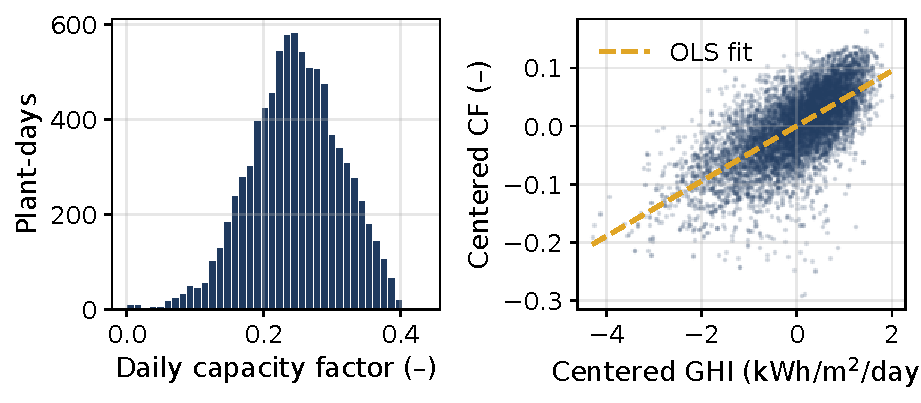
\includegraphics[width=\linewidth]{figures/eda_colombia.pdf}
\caption{Izquierda: distribución del factor de capacidad diario en los 8{,}589 días-planta. Derecha: factor de capacidad frente a la radiación global horizontal diaria de Open-Meteo (\texttt{best\_match}), ambos centrados con la media de su planta, con el ajuste por mínimos cuadrados.}
\label{fig:eda}
\end{figure}

\begin{figure}[t]
\centering
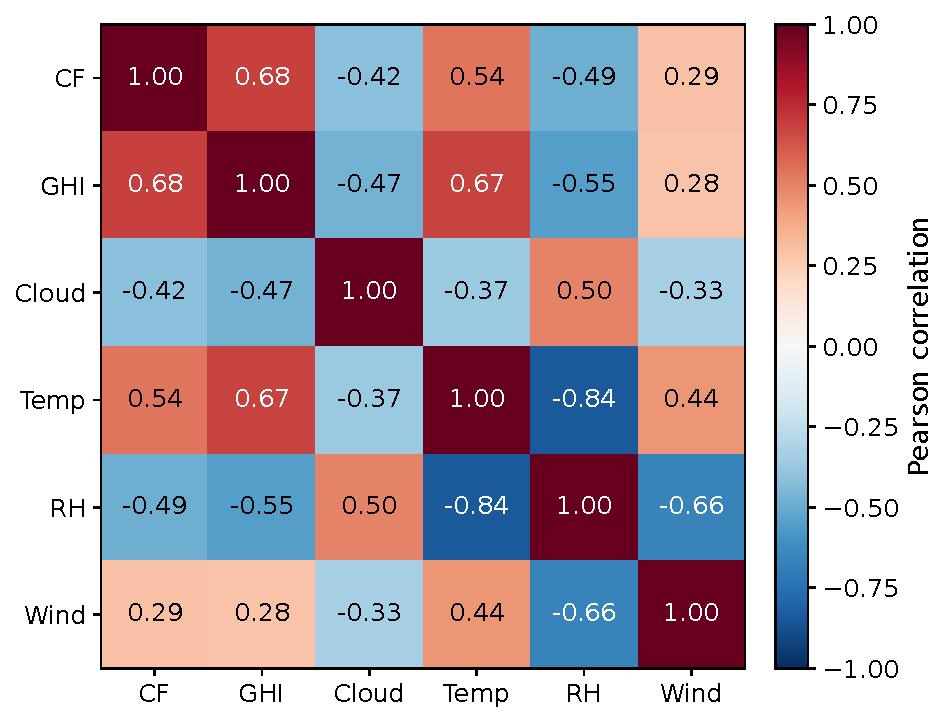
\includegraphics[width=0.7\linewidth]{figures/corr_colombia.pdf}
\caption{Correlación de Pearson entre las covariables de clima y el factor de capacidad (CF), todas centradas con la media de su planta. GHI: radiación global horizontal; Cloud: nubosidad; Temp: temperatura; RH: humedad relativa; Wind: viento.}
\label{fig:corr}
\end{figure}

% ---------------------------------------------------------------------
\subsection{Modelos de referencia (baselines)}\label{subsec:sota}

Se comparan los modelos supervisados vistos en el curso, en su implementación de scikit-learn 1.9.0 \cite{pedregosa2011sklearn}, todos con la misma entrada $\tilde{\mathbf{x}}_{pt}$ estandarizada y las mismas particiones. Se incluyen dos referencias sin clima: predecir el nivel de la planta, $\hat{y}_{pt} = \mu_p$ (equivale a $f \equiv 0$), y, en el análisis por planta, la persistencia $\hat{y}_{pt} = y_{p,t-1}$.

\textbf{Regresión lineal, Ridge y Lasso.} Estiman un modelo lineal por mínimos cuadrados, sin penalización o con penalización $\ell_2$ o $\ell_1$ \cite{hoerl1970ridge,tibshirani1996lasso}:
\begin{equation}
\hat{\boldsymbol{\beta}} = \arg\min_{\beta_0,\boldsymbol{\beta}} \sum_{i=1}^{n}\bigl(\tilde{y}_i - \beta_0 - \boldsymbol{\beta}^\top\tilde{\mathbf{x}}_i\bigr)^2 + \lambda R(\boldsymbol{\beta}), \qquad R(\boldsymbol{\beta}) = \lVert\boldsymbol{\beta}\rVert_2^2 \ \text{o}\ \lVert\boldsymbol{\beta}\rVert_1 .
\label{eq:ridge_lasso}
\end{equation}
Son la referencia natural porque la relación física entre radiación y FC es casi lineal; la penalización controla la colinealidad descrita en el EDA.

\textbf{$k$ vecinos más cercanos (KNN).} Promedia el objetivo de los $k$ puntos de entrenamiento más cercanos en distancia euclidiana \cite{cover1967nn}:
\begin{equation}
\hat{f}(\tilde{\mathbf{x}}) = \frac{1}{k}\sum_{i \in \mathcal{N}_k(\tilde{\mathbf{x}})} \tilde{y}_i .
\label{eq:knn}
\end{equation}
Representa un modelo no paramétrico que puede captar no linealidades, por ejemplo la saturación del FC en días muy soleados.

\textbf{Regresión de vectores de soporte (SVR) con kernel RBF.} Ajusta $f(\tilde{\mathbf{x}}) = \mathbf{w}^\top\phi(\tilde{\mathbf{x}}) + b$ bajo la pérdida $\varepsilon$-insensible \cite{smola2004svr}:
\begin{equation}
\min_{\mathbf{w},b}\ \frac{1}{2}\lVert\mathbf{w}\rVert_2^2 + C\sum_{i=1}^{n}\max\bigl(0,\ |\tilde{y}_i - f(\tilde{\mathbf{x}}_i)| - \varepsilon\bigr), \qquad K(\mathbf{x},\mathbf{x}') = \exp\bigl(-\gamma\lVert\mathbf{x}-\mathbf{x}'\rVert_2^2\bigr).
\label{eq:svr}
\end{equation}

\textbf{Gradient boosting por histogramas.} Como modelo flexible de árboles se usa \texttt{HistGradientBoostingRegressor}, que construye un ensamble aditivo $F_M(\tilde{\mathbf{x}}) = \sum_{m=1}^{M}\nu\, h_m(\tilde{\mathbf{x}})$, donde cada árbol $h_m$ se ajusta al gradiente negativo de la pérdida en la iteración anterior \cite{friedman2001gbm}. Se evalúa con hiperparámetros por defecto en el análisis preliminar.

\textbf{Clasificadores de la tarea complementaria.} Regresión logística multinomial, $\hat{p}_{k}(\tilde{\mathbf{x}}) = \exp(\boldsymbol{\beta}_k^\top\tilde{\mathbf{x}}) / \sum_{j}\exp(\boldsymbol{\beta}_j^\top\tilde{\mathbf{x}})$ \cite{cox1958logistic}; Naive Bayes gaussiano, que supone covariables independientes y normales dentro de cada clase \cite{hand2001idiot}; KNN con voto de los $k$ vecinos \cite{cover1967nn}; SVM lineal con probabilidades calibradas por el método de Platt \cite{cortes1995svm,platt1999probabilistic}; y SVM con kernel RBF \cite{cortes1995svm}. La referencia es la clase más frecuente.

\textbf{Hiperparámetros.} Todos los modelos se evalúan dos veces: con los valores por defecto (Ridge $\lambda=1$, Lasso $\lambda=10^{-3}$, KNN $k=25$, SVR $C=1$ y $\varepsilon=0.01$) y con búsqueda exhaustiva en rejilla dentro de la validación anidada de la Sección~\ref{subsec:config}. Las rejillas de regresión son: Ridge $\lambda \in \{10^{-3},\dots,10^{3}\}$ (7 valores); Lasso $\lambda \in \{10^{-5},10^{-4},10^{-3},10^{-2}\}$; KNN $k \in \{5,15,25,51,101\}$ con pesos uniformes o por distancia; SVR $C \in \{0.1,1,10\}$, $\varepsilon \in \{0.005,0.02\}$ y $\gamma \in \{\text{scale}, 0.1\}$. En clasificación: logística $C \in \{0.01,0.1,1,10,100\}$; Naive Bayes \texttt{var\_smoothing} $\in \{10^{-9},10^{-7},10^{-5},10^{-3}\}$; KNN igual que en regresión; SVM lineal $C \in \{0.01,0.1,1,10\}$; y SVM RBF $C \in \{0.1,1,10\}$ con $\gamma \in \{\text{scale},0.1\}$.

% ---------------------------------------------------------------------
\subsection{Modelo propuesto}\label{subsec:propuesto}

\pendiente{Esta subsección se escribe cuando el equipo defina el modelo. En el borrador del artículo el modelo aparece como ``[-]''. Debe contener, en este orden:}

\begin{enumerate}
\item \textbf{Idea central} en un párrafo: qué hace el modelo y qué problema concreto de la Sección~\ref{subsec:datos} resuelve (por ejemplo, el nivel de planta que cambia en el tiempo, la colinealidad entre covariables o la dependencia de la fuente de radiación).
\item \textbf{Formulación} con ecuaciones numeradas en la notación de la Sección~\ref{subsubsec:formulacion}: cómo produce $f(\tilde{\mathbf{x}}_{pt})$ o $\hat{y}_{pt}$ y qué pérdida minimiza.
\item \textbf{Diagrama} de la arquitectura o del flujo, en PDF vectorial generado desde \texttt{figures/make\_figures.py}.
\item \textbf{Pseudocódigo} del entrenamiento y la predicción (entorno \texttt{algorithm}).
\item \textbf{Justificación} de cada componente y qué es nuevo frente a los modelos de la Sección~\ref{subsec:sota}.
\item \textbf{Complejidad} en tiempo y memoria (por ejemplo, $O(n\,d^2)$) y número de parámetros entrenables.
\end{enumerate}

\subsubsection{Entrenamiento y optimización}

\pendiente{optimizador, regularización y criterio de parada del modelo propuesto.} Para que la comparación sea justa, sus hiperparámetros se buscan con el mismo procedimiento que los modelos de referencia: búsqueda dentro del bucle interno de la validación anidada (Sección~\ref{subsec:config}), seleccionando por $R^2$, con \pendiente{método de búsqueda, espacio explorado y número de pruebas} y un presupuesto comparable al de la rejilla más grande de los baselines (12 combinaciones por pliegue, en SVR). La semilla es 42.

% ---------------------------------------------------------------------
\subsection{Configuración experimental}\label{subsec:config}

\subsubsection{Particiones y validación anidada}

La partición se hace antes de cualquier cálculo dependiente de los datos y combina un corte temporal y uno espacial. Cada planta se divide en el tiempo: la primera mitad de sus días es su pasado, $\mathcal{T}^{\text{pas}}_p$, y la segunda mitad es su futuro, que solo se usa para medir. Además, en cada pliegue externo se deja fuera una zona completa, porque plantas a menos de 100\,km comparten el clima del día y no son independientes \cite{roberts2017cv}. Así, para la zona $z$,
\begin{equation}
\mathcal{D}^{\text{ent}}_z = \{(p,t): g(p)\neq z,\ t\in\mathcal{T}^{\text{pas}}_p\}, \qquad
\mathcal{D}^{\text{pru}}_z = \{(p,t): g(p)= z,\ t\notin\mathcal{T}^{\text{pas}}_p\},
\label{eq:particion}
\end{equation}
con $z = 1,\dots,6$. El modelo aprende del pasado de las otras zonas y se evalúa en el futuro de la zona excluida. El pasado de las plantas de la zona de prueba solo se usa para calcular su nivel $\mu_p$, $\bar{\mathbf{x}}_p$ y sus cortes de clase, y no entra al entrenamiento. El escalado estándar y la calibración de probabilidades van dentro de un \texttt{Pipeline} y se ajustan con $\mathcal{D}^{\text{ent}}_z$ \cite{kaufman2012leakage}.

Los hiperparámetros se eligen con validación anidada \cite{varma2006bias,cawley2010overfitting}. El bucle interno trabaja solo con $\mathcal{D}^{\text{ent}}_z$ y deja fuera una de las cinco zonas de entrenamiento a la vez (\emph{leave-one-group-out}); elige por $R^2$ en regresión y por F1 macro en clasificación, y reentrena con la mejor combinación sobre todo $\mathcal{D}^{\text{ent}}_z$. El bucle externo solo mide. Las predicciones de los seis pliegues externos se juntan para calcular las métricas. Como contraste, los modelos por defecto se repiten con una partición aleatoria de filas en 5 pliegues (semilla 42), donde días vecinos de una misma planta y de plantas cercanas quedan a ambos lados, para medir cuánto se infla el resultado sin el diseño anterior.

\subsubsection{Métricas}

Como el objetivo es explicar la variación diaria de cada planta, la métrica principal es el $R^2$ dentro de la planta,
\begin{equation}
R^2_p = 1 - \frac{\sum_{t}(\tilde{y}_{pt}-\hat{f}(\tilde{\mathbf{x}}_{pt}))^2}{\sum_{t}(\tilde{y}_{pt}-\bar{\tilde{y}}_p)^2},
\label{eq:r2}
\end{equation}
calculado en los días de prueba de cada planta y resumido con la mediana, el mínimo y el máximo entre las 16 plantas; un $R^2$ global premiaría acertar la diferencia de nivel entre plantas, que no es la tarea. Se reportan también el RMSE y el MAE en puntos de FC y el MAE relativo al FC medio de cada planta, $\text{MAE}^{\text{rel}}_p = \text{MAE}_p / \bar{y}_p$, promediado entre plantas, que permite comparar plantas de distinto nivel. En clasificación se reportan F1 macro, exactitud, exactitud balanceada, precisión y exhaustividad macro, AUC-ROC macro uno contra el resto \cite{fawcett2006roc} y kappa de Cohen con ponderación cuadrática \cite{cohen1968kappa}, que penaliza más confundir un día bajo con uno alto que con uno medio.

\subsubsection{Pruebas estadísticas}

Con 16 plantas en 6 zonas, la unidad de muestreo es la planta y no el día. Los intervalos de confianza del 95\,\% de la mediana de $R^2_p$ se obtienen remuestreando plantas con reemplazo (bootstrap por conglomerados, 5{,}000 réplicas) \cite{field2007bootstrap}. Las diferencias entre dos modelos se prueban con la prueba de rangos con signo de Wilcoxon sobre las 16 diferencias pareadas por planta \cite{wilcoxon1945}. Con 16 pares la prueba tiene poca potencia y, al no haber una hipótesis confirmatoria previa, los valores $p$ se reportan sin corrección por comparaciones múltiples y se leen como evidencia exploratoria.

\subsubsection{Estudio de ablación}

Cada variante cambia un solo componente y se evalúa con el mismo protocolo y la misma métrica principal que el modelo completo:
\begin{itemize}
\item \textbf{Covariables:} solo radiación frente a las cinco variables, para probar si nubosidad, temperatura, humedad y viento aportan información además de la radiación, dada su colinealidad.
\item \textbf{Fuente de radiación:} \texttt{best\_match} frente a \texttt{era5}, para medir cuánto del techo del resultado depende del producto de clima y no del modelo \cite{urraca2018era5ghi}.
\item \textbf{Corrección física:} radiación frente al índice corregido por temperatura de celda, para probar si la pérdida térmica genérica mejora la predicción.
\item \textbf{Decisiones de la base:} sin excluir la puesta en marcha, con otra duración de exclusión e incluyendo ALMA II, para verificar que el resultado no depende de esos filtros.
\item \textbf{Diseño de validación:} partición aleatoria frente a zona fuera y futuro de la planta, para cuantificar la fuga espacial y temporal.
\item \textbf{Componentes del modelo propuesto:} \pendiente{una variante por cada componente que se quite o se reemplace, con la hipótesis que pone a prueba.}
\end{itemize}

\subsubsection{Software, hardware y tiempo de cómputo}

Los experimentos usan Python 3.11, scikit-learn 1.9.0, pandas 2.3, NumPy 2.3 y SciPy 1.16 (entorno completo en \texttt{environment.yml}). El tiempo de cómputo de cada modelo se mide como el tiempo de reloj de todo el protocolo (seis pliegues externos, incluida la búsqueda interna), con búsqueda paralela en todos los núcleos disponibles. Hardware: \pendiente{procesador, memoria y sistema operativo}. Como la partición es determinista y todos los modelos estocásticos usan la semilla 42, cada configuración se ejecuta una vez; la variabilidad se reporta entre plantas y con el bootstrap descrito arriba.

% =====================================================================
\section{Resultados}\label{sec:resultados}

\begin{instruccion}
Tabla comparativa del modelo propuesto contra todos los modelos de referencia con la métrica principal y el tiempo de cómputo; al menos una figura de apoyo; y la prueba estadística frente a cada modelo. No repitas en el texto los números exactos de la tabla.
\end{instruccion}

% =====================================================================
\section{Conclusiones}\label{sec:conclusiones}

\begin{instruccion}
Entre 1 y 2 párrafos: si se cumplió el objetivo frente a los modelos de referencia en error y tiempo de cómputo, limitaciones del estudio y trabajo futuro.
\end{instruccion}

\backmatter

\section*{Declaraciones}

\begin{itemize}
\item \textbf{Disponibilidad de datos:} la base \texttt{tabla\_diaria\_colombia.csv} se construye con datos públicos de XM \cite{xm_api}, Open-Meteo \cite{zippenfenig2023openmeteo} y Global Energy Monitor \cite{gem2026solar}, y se regenera con el cuaderno \texttt{Clima\_a\_Generacion\_Colombia.ipynb}. \pendiente{enlace público a los CSV, que no están en el repositorio por su tamaño.}
\item \textbf{Disponibilidad de código:} \url{https://github.com/AlexT09/ModelSolar}, carpeta \texttt{notebooks} (cuadernos \texttt{Clima\_a\_Generacion\_Colombia.ipynb} y \texttt{Benchmark\_Colombia.ipynb}). Semilla 42.
\item \textbf{Contribución de los autores:} \pendiente{contribución de cada autor.}
\item \textbf{Conflicto de intereses:} los autores declaran no tener conflictos de interés.
\end{itemize}

\bibliography{sn-bibliography}

\end{document}
